\documentclass{standalone}
\usepackage{tikz}
\usepackage{amsmath}

\begin{document}

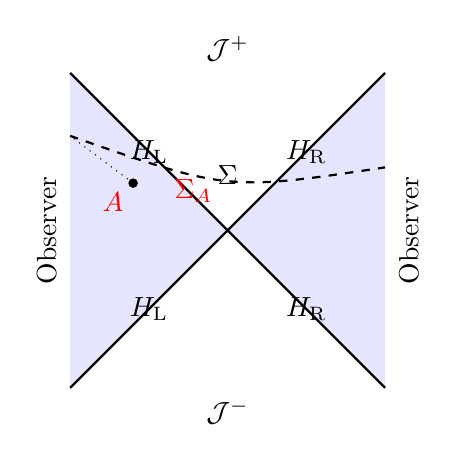
\begin{tikzpicture}

% Define colors
\colorlet{lightblue}{blue!10}

% Define coordinates
\coordinate (O) at (0,0);
\coordinate (A) at (-1.2,0.6);

% Draw the static patches
\fill[lightblue] (-2,-2) -- (0,0) -- (-2,2) -- cycle;
\fill[lightblue] (2,-2) -- (0,0) -- (2,2) -- cycle;

% Draw the main lines
\draw[thick] (-2,-2) -- (0,0) -- (2,-2);
\draw[thick] (-2,2) -- (0,0) -- (2,2);

% Draw the dashed spacelike slice
\draw[dashed, thick] (-2,1.2) .. controls (0,0.5) .. (2,0.8);

% Draw the lightcone and labels
\draw[dotted] (A) -- (-2,1.2);
\node[red, right] at (-0.8,0.5) {$\Sigma_A$};
\node[red, below left] at (A) {$A$};
\filldraw[black] (A) circle (1.5pt);

% Draw the cosmological horizons
\node at (-1,1) {$H_{\rm L}$};
\node at (1,1) {$H_{\rm R}$};
\node at (-1,-1) {$H_{\rm L}$};
\node at (1,-1) {$H_{\rm R}$};

% Label observers
\node[rotate=90] at (-2.3,0) {Observer};
\node[rotate=90] at (2.3,0) {Observer};

% Label future and past infinity
\node at (0,2.3) {$\mathcal{J}^+$};
\node at (0,-2.3) {$\mathcal{J}^-$};

% Label slice
\node at (0,0.7) {$\Sigma$};

\end{tikzpicture}

\end{document}